\documentclass[letterpaper]{article}
\usepackage{amssymb}
\usepackage{fullpage}
\usepackage{amsmath}
\usepackage{epsfig,float,alltt}
\usepackage{psfrag,xr}
\usepackage[T1]{fontenc}
\usepackage{url}
\author{Prof. Grizzle}
\title{Rob 501 - Mathematics for Robotics\\
HW \#4}

\begin{document}
\date{}
\maketitle


 \newcommand{\trace}{\mathrm{trace}}
\newcommand{\real}{\mathbb R}  % real numbers  {I\!\!R}
\newcommand{\nat}{\mathbb N}   % Natural numbers {I\!\!N}
\newcommand{\cp}{\mathbb C}    % complex numbers  {I\!\!\!\!C}
\newcommand{\ds}{\displaystyle}
\newcommand{\mf}[2]{\frac{\ds #1}{\ds #2}}
\newcommand{\Nagy}[2]{{Nagy, Page~#1, }{Prob.~#2}}
\newcommand{\spanof}[1]{\textrm{span} \{ #1 \}}
\parindent 0pt


\begin{flushright}
{\bfseries Due Oct. 4, 2018} \\
{\bfseries 3PM via Gradescope} \\[3mm]
\end{flushright}

\noindent \textbf{Reading Assignment:}  Chapters 6 and 7 of Nagy.


\begin{enumerate}


%Prob. 1 Representation and change of basis matrix
\item \Nagy{136}{4.4.3} (Nagy's ``ordered bases'' are simply called bases in lecture. Finding the components is what we call finding the representation).  In addition, find the change of basis matrix $P$ from the basis $\cal S$ to the basis $\cal Q$.

%so that for every polynomial $p \in {\mathbb P}_2$,
%    $$ [p]_{\cal Q} = P [p]_{\cal S}$$
%    where $ [p]_{\cal Q}$ is the representation of the polynomial $p$ in the basis $\cal Q$ and $[p]_{\cal S}$ is the representation of the polynomial $p$ in the basis $\cal S$.

%Prob. 2 e-values and e-vectors
\item Calculate by hand a set of e-vectors of the matrix $A_3$ below (It is noted
that the e-values are obvious since the matrix is upper triangular.)
$$A_3=\left[ \begin{array}{ccc} 1 & 4 & 10 \\ 0 & 2 & 0 \\ 0& 0& 3 \end{array} \right] $$
Verify that the e-vectors you computed are linearly independent. \\

\textbf{Remark:} Check you answers in MATLAB.  We noted in lecture that e-vectors are not unique. Do your e-vectors agree with those computed by MATLAB using the \texttt{eig} command?

%Prob. 3 e-values and e-vectors
\item For the matrix $A_4$ below, compute its e-values and e-vectors.
 $$A_4=\left[ \begin{array}{ccc} 3 & 1 &0 \\ 0 & 3 & 0 \\ 0& 0& 2 \end{array} \right] $$
 Can you find a basis for $\real^3$ consisting of e-vectors?

 %Prob. 4 Similar matrices
\item Two square matrices $A$ and $B$ are said to be \textbf{similar} if there exists an invertible matrix $P$ such that
$B=P^{-1}AP$. Show that if $A$ and $B$ are similar matrices, then
they have the same characteristic equation, and hence the same
eigenvalues. \textbf{Note:} The characteristic polynomial of a
square matrix $A$ is $\det \left( \lambda I - A \right)$; the
characteristic equation is $\det \left( \lambda I - A \right)=0$.\\


%Prob. 5 Similarity
\item For the matrix $A_3$ in Prob. 2 above, show that $A$ is similar to a diagonal matrix. You can use results from lecture.

%Prob. 6 Matrix Representation
\item Let ${\mathcal F}=\real$ and let $\cal X$ be the set of $2 \times 2$ matrices with real coefficients. Define $L:{\cal X} \to {\cal  X}$ by
$$ L(M) = \frac{1}{2}( M+M^\top),$$
where $M\in {\cal X}$ is a $2 \times 2$ real matrix.

\begin{enumerate}
\setlength{\itemsep}{.1in}
\renewcommand{\labelenumi}{(\alph{enumi})}
\item Show that $L$ is a linear operator.

\item Compute $A$, the matrix representation of $L$, when the basis
$$ E^{11} = \left[ \begin{array}{cc} 1 & 0  \\ 0& 0 \end{array} \right],  E^{12} = \left[ \begin{array}{cc} 0 & 1  \\ 0& 0 \end{array} \right],  E^{21} = \left[ \begin{array}{cc} 0 & 0  \\ 1& 0 \end{array} \right],  E^{22} = \left[ \begin{array}{cc} 0 & 0  \\ 0& 1 \end{array} \right]$$
is used on both copies of $\cal X$ (i.e., on both the domain and codomain of $L$).

\end{enumerate}

% 7 Matrix Representation
\item  Let $A$ be an $n \times n$ matrix with possibly complex coefficients. Let $L: {\cp^n} \to {\cp}^n$ by $L(x) = Ax$. Note that the field is $\mathcal{F} = \cp$.

    \begin{enumerate}
\setlength{\itemsep}{.1in}
\renewcommand{\labelenumi}{(\alph{enumi})}

\item Compute the matrix representation of $L$ when the ``natural'' (also called canonical) basis is used in ${\cp}^n$.  Call your representation $\hat A$ and find its relation to the original matrix $A$.

\item  Suppose that the e-values of $A$ are distinct. Compute the matrix representation $L$ with respect to a basis constructed from the e-vectors of $A$. Call your representation $\hat A$.

\end{enumerate}


% 8 regression, phony data
\item Read the handout on `Linear Regression' and then work this problem. We will be developing the theoretical basis for the handout in lecture. In the meantime, it is instructive to ``play'' with the ideas a bit.

\begin{figure}[h!]
\centering
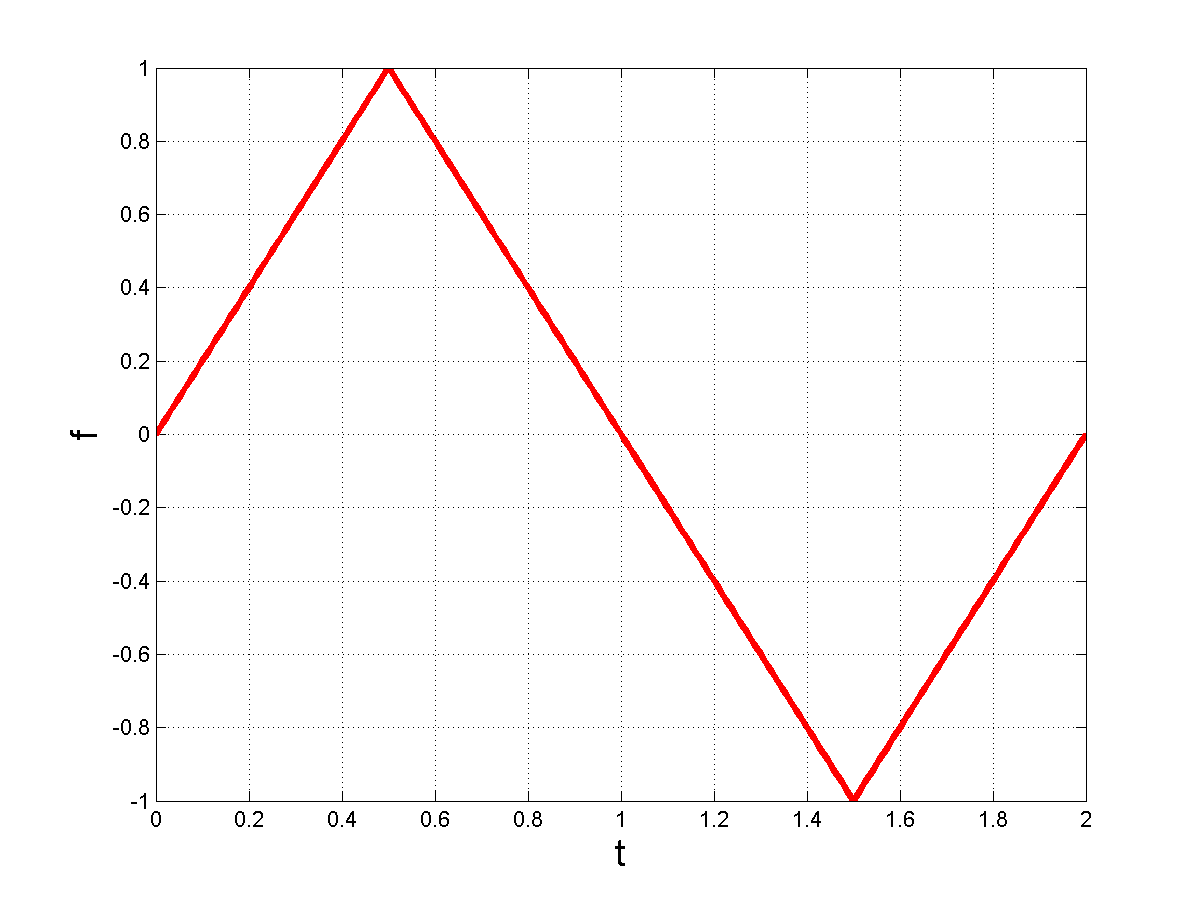
\includegraphics[width=0.5\textwidth]{MATLAB/Prob8TriWave.png}
\caption{Triangle Wave for Problem 8}
\end{figure}

\begin{enumerate}
\setlength{\itemsep}{.1in}
\renewcommand{\labelenumi}{(\alph{enumi})}
\item From the MATLAB folder on CANVAS, download the file \texttt{HW04\_Prob8\_Data.mat}. Load the data into the MATLAB workspace with the following command
    \begin{verbatim}
>> load HW04_Prob8_Data
>> % This makes the plot
>> plot(t,f,'r','linewidth',3)
>> grid on
>> xlabel('t','FontSize',18)
>> ylabel('f','FontSize',18)
>> print Prob8TriWave -dpng
    \end{verbatim}
    There is nothing to turn in for this part of the problem.

\item Compute a least squares fit of the data to $\{ 1, t, t^2, t^3, t^4, t^5\}$. As in the handout, build your basis vectors by evaluating the functions $t^k$ at the provided time points. Turn in the coefficients you obtain and a plot of your fit versus the function. Do not turn in your code.

    \item Repeat the fitting process, but this time use the functions $\{\sin(\pi t), \sin(2 \pi t), \cdots, \sin(5 \pi t) \}$. Turn in the coefficients you obtain and a plot of your fit versus the function.  To be clear, you are seeking $\alpha_k$ to minimize the error of $$||f - \sum_{k=1}^{5} \alpha_k \sin(k \pi t) ||^2$$

\end{enumerate}

% 9 regression noisy data
\item  From the MATLAB folder on CANVAS, download the file \texttt{HW04\_Prob9\_Data.mat}. Fit a set of functions to the data; to be clear, you get to chose your favorite functions for the regression. Report the functions you used, the coefficients you obtained, and a plot of your fit versus the function. In addition, from your fit, estimate the derivative of the function $f(t)$ at $t=0.3$. (Differentiate the function you fit to the data) \textit{Do not obsess over this. It is meant to be fun, not a burden! It should be very easy to modify your MATLAB code from Prob. 8 for a solution to this problem.}


\begin{figure}[h!]
\centering
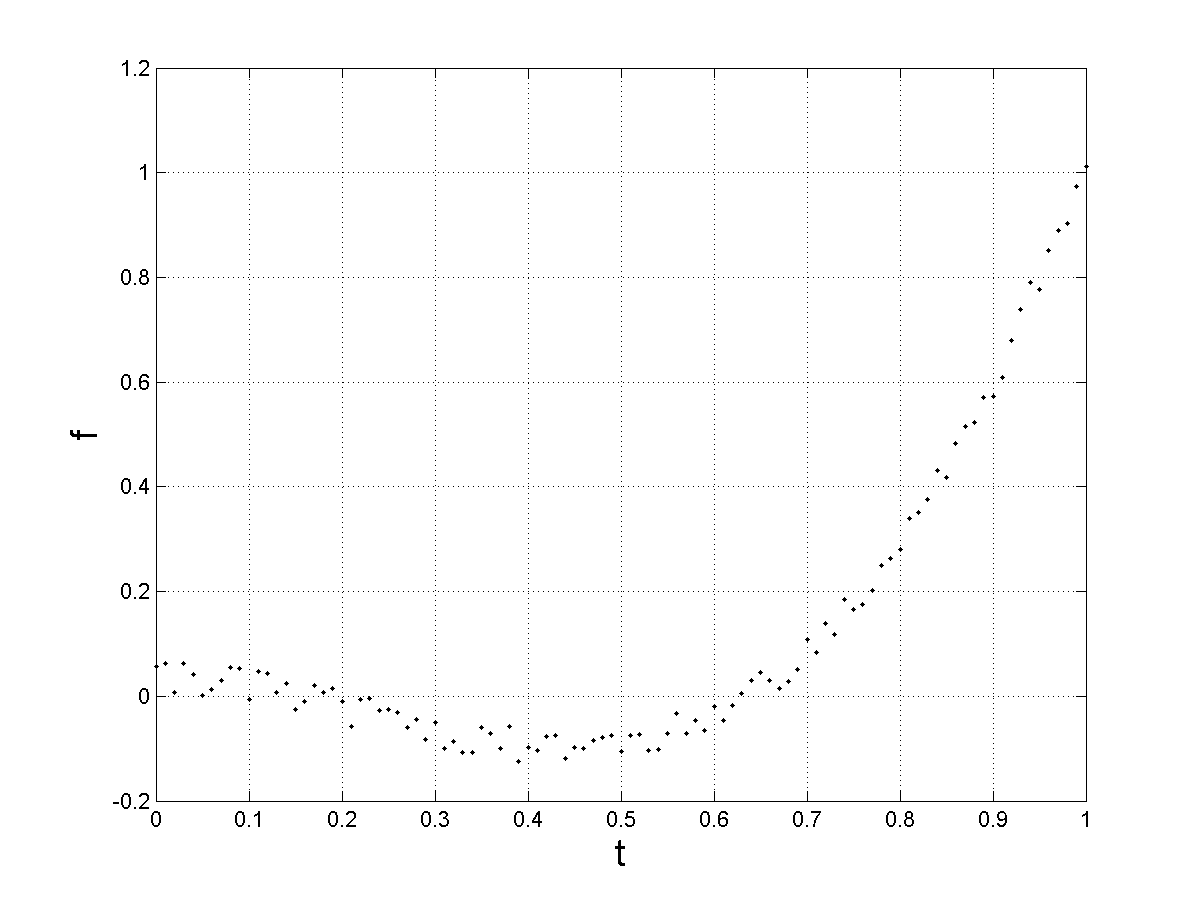
\includegraphics[width=0.5\textwidth]{MATLAB/Prob9NoisyData.png}
\caption{Noisy Data for Problem 9}
\end{figure}


%
%%Prob. 7 Matrix representation
%\item   Let ${\mathcal F}=\real$, let $\cal X$ be the set of polynomials with real coefficients and degree less than or equal to two and . let $\cal Y$ be the set of polynomilas with degree less than or equal to one. Similar to lecture, define $L:{\cal X} \to {\cal  Y}$ by $L(p(t)) = \frac{d}{dt} p(t)$. Compute the matrix representation $L$ when the basis for $\cal X$ is $\{ 1, 2t, 4t^2-2\}$ and the basis for $\cal Y$ is $\{ 4, 2t \}$
%


%End of list of HW Problems
\end{enumerate}

\newpage

\begin{center}
{\bf Hints}
\end{center}

\noindent \textbf{Hints: Prob. 1} Recall that the change of basis matrix \textbf{from} the basis $\{ v^1, \ldots, v^n\}$ \textbf{to} the basis $\{ \tilde{v}^1, \ldots, \tilde{v}^n\}$ is the $n \times n$ matrix $P$ with $i$-th column given by
$$ P_i = [v^i]_{\tilde{v}},$$
the representation of $v^i$ in the basis $\{ \tilde{v}^1, \ldots, \tilde{v}^n\}$,
and the  change of basis matrix \textbf{from} the basis $\{ \tilde{v}^1, \ldots, \tilde{v}^n\}$  \textbf{to} the basis $\{ v^1, \ldots, v^n\}$ is the $n \times n$ matrix $\tilde{P}$ with $i$-th column given by
$$ \tilde{P}_i = [\tilde{v}^i]_{v}.$$
Moreover, $P \tilde{P} = \tilde{P} P = I$, the $n\times n$ identity matrix. Consequently, you should always compute whichever of the two matrices is easier, and then get the other by matrix inversion in MATLAB.

\vspace{1cm}

\noindent \textbf{Hints: Prob. 3} The answer is NO, you cannot find such a basis The matrix is ``defective'' (check definition of defective matrix on the web), meaning it does not have a full set of e-vectors. To treat such matrices, one has to learn about the Jordan canonical form, a subject we will not cover in ROB 501. The point of the problem is simply that when e-values are not distinct, you may not have enough e-vectors to build a basis.  Jordan canonical forms are treated in EECS 560 = ME 564 = AERO 550.\\

\vspace{1cm}

\noindent \textbf{Hints: Prob. 4} Recall that for compatible square matrices $A$ and $B$, $\det(AB) = \det(A) \det(B)$.\\

\vspace{1cm}

\noindent \textbf{Hints: Prob. 5} Translate the equation $A v^i = \lambda_i v^i$ into an equation involving matrices
$$P = [v^1~|\cdots~ | v^n] ~~ \mbox{and} ~~  \Lambda = \mathrm{diag} (\lambda_1, \cdots , \lambda_n) $$
where in this problem, $n=3$. Questions to ask yourself: Is $P$ invertible? And which is correct, $AP = \Lambda P$ or
$AP = P \Lambda $? Perhaps neither?
\vspace{1cm}

\noindent \textbf{Hints: Prob. 6}  $A$ will be $4 \times 4$. From lecture, we have a formula for the columns of $A$. \\

\vspace{1cm}

\noindent \textbf{Hints: Prob. 7} In both parts, you are using the same basis on the domain and the co-domain of $L$.  The point of (a) is that when you view a matrix as linear operator, and write $L(x) = Ax$, you are using the natural basis on ${\cal F}^n$. The answer for (b) will show that $A$ is similar to a diagonal matrix, viz Prob.~5, though the perspective is different.

\vspace{1cm}

\noindent \textbf{Hints: Prob. 8 and 9}
For your convenience $t$ and $f$ are given as column vectors in the data file.
An easy way in MATLAB to obtain a column of $1$'s the same length as $t$ is $1+0*t$. There are many other ways too!
If you're using python instead of MATLAB, you can load the .mat files with the package scipy.io.loadmat (\url{https://docs.scipy.org/doc/scipy-0.19.0/reference/generated/scipy.io.loadmat.html}).

\end{document}


